%% LyX 2.2.4 created this file.  For more info, see http://www.lyx.org/.
%% Do not edit unless you really know what you are doing.
\documentclass[english]{article}
\usepackage{lmodern}
\usepackage[T1]{fontenc}
\usepackage[latin9]{inputenc}
\usepackage{geometry}
\geometry{verbose,tmargin=3cm,bmargin=3cm,lmargin=2.5cm,rmargin=2.5cm}
\usepackage{textcomp}
\usepackage{graphicx}
\newcommand\at[2]{\left.#1\right|_{#2}}
\usepackage{amssymb}
\usepackage{amsmath}


\makeatletter

%%%%%%%%%%%%%%%%%%%%%%%%%%%%%% LyX specific LaTeX commands.
%% Because html converters don't know tabularnewline
\providecommand{\tabularnewline}{\\}

\makeatother

\usepackage{babel}
\begin{document}

\title{3F8: Inference\\
 Full Technical Report}

\author{Danut-Gabriel Buica}
\maketitle
\begin{abstract}

Dealing with high dimensions, we can easily linearly separate our data. This may lead to overfitting, therefore,  we want to further improve our Logistic Classifier by applying Laplace approximation on our weigths. This will prevent the classification to be made with too high certainty while still minimizing the misclassification. we will also investigate the performance of selecting hyper-parameter values by optimizing the model evidence. By experimated with different parameters, we determined that using a trade-off between minimizing the data misfit and model complexity, we can achive far better prediction rates.

\end{abstract}

\section{Introduction}
\begin{enumerate}
	
\item During our coursework we implemented a Logistic Classifier. The problem is that in higher dimmension our data can be liniarly separated by many set of weights and in some cases this may lead to overfitting.
\item To solve this problem we will implement a Bayesian binary classifier that applies the Laplace approximation to our Logistic Classification model. Furthermore, we will investigate the performance of selecting hyper parameters values by optmizing over the model evidence.
\end{enumerate}

\section{Exercise a)}\label{a}

The goal of the Laplace approximation is to fit a Gaussian approximation to a probability density defined over a set of continuous variables. 
First, we will consider the case of a single continuous variable $ z $ with the probability distribution $ p(z) $ so that:
\begin{equation}\label{1}
	p(z) = \frac{1}{Z} f(z)
\end{equation}
where $ Z = \int f(z) dz $ is the unknown normalization constant. Let $ q(z) = \mathcal{N} (z|m, v) $ denote our Gaussian approximation. We want our Gaussian to be centered on a mode of $ p(z) $. Therefore, $ m $ is the MAP solution of $ p(z) $:
\begin{equation}\label{2}
	\at{\frac{df(z)}{dz}}{z=m} = 0
\end{equation}

As for finding the value of $ v $, the property of a Gaussian distribution that its logarithm is a quadratic function
of the variables proves to be very useful. By considering the Taylor expansion of $ ln f(z) $ around $ m $, we get:
\begin{equation}\label{3}
	\ln f(z) \approx \ln f(m) - \frac{1}{2} A (z-m)^2
\end{equation}
where
\begin{equation}\label{4}
	A = - \at{\frac{d^2}{dz^2} \ln f(z)}{z=m}
\end{equation}
Notice that the first order of the Taylor expnasion is $ 0 $ since $ m $ is the local maximum of the distribution. By taking the exponential of eq. \ref{3} we obtain:
\begin{equation}\label{5}
	f(z) \approx f(m) \exp \left( - \frac{A}{2} (z-m)^2\right ) = f(m) \left( \frac{A}{2 \pi}\right)^{-1/2} \mathcal{N}(z|m, A^{-1})
\end{equation}

Thus, we get the following forms of $ q(z) = \mathcal{N}(z|m, A^{-1}) $ and $ Z =  f(m) \left( \frac{A}{2 \pi}\right)^{-1/2} $.
We should note that this is well defined when $ A > 0 $, in other words $ m $ represents a local maximum. 

Furthermore, we can extend the Laplace approximation to a distribution $ p(\mathbf{z}) = \frac{1}{Z} f(\mathbf{z})$ defined over an $ M $-dimensional space $ \mathbf{z} $. Our choice for the mean of the Gaussian will again the MAP solution $ \mathbf{z}_{MAP} $ with the property that:
\begin{equation}\label{irststderivative}
	\at{\nabla f(\mathbf{z})}{\mathbf{z} = \mathbf{z}_{MAP}} = 0
\end{equation}

Hence, expanding $ \ln f(\mathbf{z}) $ around $ \mathbf{z}_{MAP}$ gives:
\begin{equation}\label{taylor}
	\ln f(\mathbf{z}) \approx \ln f(\mathbf{z}_{MAP}) - \frac{1}{2}(\mathbf{z} - \mathbf{z}_{MAP})^T\mathbf{A}(\mathbf{z} - \mathbf{z}_{MAP})
\end{equation}
where $ \mathbf{A} $ is an $ M \times M $ Hessian matrix defined as:
\begin{equation}\label{hessian}
	\mathbf{A} = - \at{\nabla \nabla \ln f(\mathbf{z})}{\mathbf{z} = \mathbf{z}_{MAP}} 
\end{equation}

By taking the exponential of eq. \ref{taylor} we obtain:
\begin{equation}\label{f}
	f(\mathbf{z}) \approx f(\mathbf{z}_{MAP}) \exp\left(- \frac{1}{2}(\mathbf{z} - \mathbf{z}_{MAP})^T\mathbf{A}(\mathbf{z} - \mathbf{z}_{MAP})\right) = f(\mathbf{z}_{MAP}) \frac{(2 \pi)^{M/2}}{|\mathbf{A}|^{1/2}} \mathcal{N}(\mathbf{z}|\mathbf{z}_{MAP}, \mathbf{A}^{-1})
\end{equation}

This gives us $ q(\mathbf{z}) = \mathcal{N}(\mathbf{z}|\mathbf{z}_{MAP}, \mathbf{A}^{-1}) $ and 
\begin{equation}\label{zed}
	Z = f(\mathbf{z}_{MAP}) \frac{(2 \pi)^{M/2}}{|\mathbf{A}|^{1/2}}
\end{equation}

Note that $ \mathbf{A} $ must be positive definite for a local maximum at $ \mathbf{z}_{MAP} $.

We go on with how to apply the theory on Laplace approximation to the Logistic classifier. We firstly assume the prior on our weights to be of the following form:
\begin{equation}\label{weights_prior}
	p(\mathbf{w}) = \mathcal{N}(\mathbf{w}|\mathbf{m}_0, \mathbf{S}_0)
\end{equation}

Hence for a dataset $ \mathcal{D}(\mathbf{y}, \mathbf{\tilde{X}}) $ the posterior distribution over $ \mathbf{w} $ will be:
\begin{equation}\label{post}
	p(\mathbf{w}|\mathcal{D}) \propto p(\mathbf{w}) p(\mathcal{D}|\mathbf{w})
\end{equation}

From the central limit theorem, we know that the posterior distribution is expected to become better approximated by a Gaussian as the number of data points observed increases. Therefore, we will use Laplace approximation to find $ q(\mathbf{w}) = \mathcal{N}(\mathbf{w}|\mathbf{w}_{MAP}, \mathbf{S}_N) \simeq p(\mathbf{w}|\mathcal{D}) $. In this case, $ f(\mathbf{w}) = p(\mathbf{w}) p(\mathcal{D}|\mathbf{w}) $.

By taking the logarithm of $ f(\mathbf{w}) $ and substituting the prior and the log-likelihood, we obtain:

\begin{equation}\label{negative_log}
	f(\mathbf{w}) = - \frac{1}{2} (\mathbf{w}-\mathbf{m}_0)^T \mathbf{S}_0^{-1}(\mathbf{w}- \mathbf{m}_0) + \sum_{n=1}^{N}[y_n \ln(\sigma(\mathbf{w}^T \tilde{X}_n)) - (1 - y_n) \ln (1 - \sigma(\mathbf{w}^T \tilde{X}_n)] + const
\end{equation}

We then proceed on finding $ \mathbf{w}_{MAP} $ by maximizing $ f(\mathbf{w}) $. The covariance matrix is given by the inverse of the second derivative of the log-likelihood as follows:

\begin{equation}\label{cavariance}
	\mathbf{S}_N^{-1} = - \at{\nabla \nabla\ln f(\mathbf{w})}{\mathbf{w} = \mathbf{w}_{MAP}} = \mathbf{S}_0^{-1} + \sum_{n=1}^{N} \sigma(\mathbf{w}^T \tilde{X}_n)(1-\sigma(\mathbf{w}^T \tilde{X}_n))\tilde{X}_n\tilde{X}_n^T
\end{equation}

The predictive distibution for a $ \mathcal{C}_1 $ for a new feature vector $ \phi $ is obatained by marginalizing with respect to the posterior distribution $ p(\mathbf{w}|\mathcal{D})  $:

\begin{equation}\label{class1}
	p(\mathcal{C}_1 | \phi, \mathcal{D}) = \int p(\mathcal{C}_1 | \phi, \mathbf{w}) p(\mathbf{w}|\mathcal{D}) d\mathbf{w} \simeq \int
	\sigma(\mathbf{w}^T \phi) q(\mathbf{w}) d\mathbf{w}
\end{equation}

Note that $ 	p(\mathcal{C}_2 | \phi, \mathcal{D}) = 1 - 	p(\mathcal{C}_1 | \phi, \mathcal{D}) $ . Given that $ \sigma(\mathbf{w}^T \phi) $ depends only on the projection of $ \mathbf{w} $ onto $ \phi $, let $ a = \mathbf{w}^T \phi $.  This gives:

\begin{equation}\label{delta}
	\sigma(\mathbf{w}^T \phi) = \int \delta (a - \mathbf{w}^T \phi) \sigma(a) d a
\end{equation}

Substituting \ref{delta} in \ref{class1} and denoting $ p(a) = \int \delta (a - \mathbf{w}^T \phi) q (\mathbf{w}) d \mathbf{w} $, we can rewrite the predictive distribution as:
\begin{equation}\label{4.147}
		p(\mathcal{C}_1 | \phi, \mathcal{D}) = \int \sigma(a) p(a) da
\end{equation} 

We can view, the delta function as a distribution $ g(a|\mathbf{w}) = \mathcal{N}(a, 0) $. Thus, $ p(a) $ is a marginal distribution from a joint distribution $ q(\mathbf{w}) $, therefore also a Gaussian for which we can calculate the mean $ \mu_a $ and variance $ \sigma_a^2 $ using moments.

\begin{equation}\label{mean}
	\mu_a = \mathbb{E}[a] = \int p(a) a da = \int q(\mathbf{w}) \mathbf{w}^T \phi d(\mathbf{w}) = \mathbf{w}_{MAP}^T \phi
\end{equation}

\begin{equation}\label{variance}
	\sigma_a^2 = \mathbb{V}[a] = \int p(a) (a^2 - \mathbb{E}[a]^2)da
	= \int q(\mathbf{w})((\mathbf{w}^T \phi)^2- (\mathbf{w}_{MAP}^T \phi)^2) d\mathbf{w} = \phi^T \mathbf{S}_N \phi
\end{equation}

Hence,

\begin{equation}\label{class1pred}
	p(\mathcal{C}_1|\mathcal{D}) = \int \sigma(a) \mathcal{N}(a|\mu_a, \sigma_a^2) da
\end{equation}

By making use of the similarity between the logistic sigmoid and the probit funtion $ \sigma(a) \simeq \Phi(\lambda a) $ with $ \lambda^2 = \pi / 8 $, we can rewrite eq. \ref{class1pred} as follows:

\begin{equation}\label{probit1}
	p(\mathcal{C}_1|\mathcal{D}) = \int \Phi(\lambda a) \mathcal{N}(a|\mu_a, \sigma_a^2) da = \Phi \left(\frac{\mu_a}{\sqrt{\lambda^{-1/2} + \sigma_a^2 }}\right)
\end{equation}

Moreover, by defining $ \kappa(\sigma^2) = \sqrt{(1 - \pi \sigma^2 / 8)^{-1}} $, the above equation becomes:

\begin{equation}\label{final}
	p(\mathcal{C}_1|\mathcal{D}) = \sigma(\kappa(\sigma_a^2)\mu_a)
\end{equation}

We can see that when $ \mu_a = 0 $ the decision boundary corresponds to $ p(\mathcal{C}_1|\mathcal{D}) = 0.5 $ and it is the same boundary as the one obtained by using $ \mathbf{w}_{MAP} $. The decision boundary of Laplace approximation is the same as the decision boundary of the MAP estimator as both minimize the number of misclassifications. Therefore, we expect the same values for the confusion matrices, but different log-likelihoods.  We expect the Laplace log-lokelihoods to be smaller as it tries to avoid overfitting.
 
We continue by computing the model evidence of the Bayesian model ($ Z = p(\mathcal{D}) $). We have our dataset $ \mathcal{D} $, a set of models $ \mathcal{M} $ having parameters $ \{\mathbf{w}_i\} $:

\begin{equation}\label{model}
	Z = p(\mathcal{D}) = \int f(\mathbf{w}) d \mathbf{w} = \int p(\mathcal{D}|\mathbf{w}) p(\mathbf{w}) d\mathbf{w}
\end{equation}

By applying \ref{zed} we obtain the following:

\begin{equation}\label{lnmodel}
	\begin{split}
		\ln p(\mathcal{D}) &\simeq \ln p(\mathcal{D}|w_{MAP}) + \ln p(\mathbf{w}_{MAP}) + \frac{M}{2} \ln(2 \pi ) + \frac{1}{2} \ln|\mathbf{S}_N| \\
		&\simeq \ln p(\mathcal{D}|w_{MAP}) - \frac{1}{2} (\mathbf{w}_{MAP} - \mathbf{m}_0)^T \mathbf{S}_0^{-1} (\mathbf{w}_{MAP} - \mathbf{m}_0) + \frac{1}{2} \ln|\mathbf{S}_N| +\frac{1}{2} \ln|\mathbf{S}_0|
	\end{split}
\end{equation}

The first term in the first line represents the log-likelihood evaluated at the MAP solution and the other three terms represent the "Occam factor" which penalises the model complexity. The model complexity depends on the number of the parameters and also on the prior that we assigned. Te best evidence is achieved by a trade-off between data misfit minimization and model complexity minimization. 
For the prior stated in the exercise we set $ \mathbf{m}_0 = 0 $ and $ \mathbf{S}_0 = \sigma_0^2 \mathbf{I} $.

\section{Exercise b)}

To find the MAP solution, we performed gradient based minimization using the python funcion
\newline \verb|scipy.optimize.fmin_l_bfgs_b|. For this we give it as an argument for the gradient the Jacobian:

\begin{equation}\label{jacobian}
	\frac{dp(\mathbf{w}|\mathcal{D})}{d\mathbf{w}} = \mathbf{w}^T \mathbf{S}_0^{-1} + \mathbf{X}^T[\mathbf{y} - \sigma(\mathbf{w}^T\mathbf{X})]
\end{equation}

The code to train and fit the weights on a Gaussian with mean $ \mathbf{w}_{MAP} $ and covariance $ \mathbf{S}_N $ and to compute the model evidence based on the above theory (eq. \ref{lnmodel}) can be seen below. Note the use of Cholesky factorization to optimise the calculation of the determinants.

\begin{verbatim}
def logf(params, *args):
    #compute the negative log-likelihood
    w = params
    X_tilde_train = args[0]
    y_train = args[1]
    S_0_inv = args[2]
    sigmoid = predict(X_tilde_train,w)
    answer = np.dot(y_train, np.log(sigmoid)) + np.dot((1-y_train),np.log(1-sigmoid))
    answer = answer - 0.5*np.dot(np.matmul(w, S_0_inv), w)
    return (-answer)

def logfprime(params, *args):
    #compute Jacobian
    w = params
    X_tilde_train = args[0]
    y_train = args[1]
    cov_0_inv = args[2]
    sigmoid_value = predict(X_tilde_train,w)
    answer = np.dot(cov_0, w) - np.dot(np.transpose(X_tilde_train), (y_train - sigmoid_value))
    return answer

def compute_hessian(X_tilde, w, var):
    sigmoid = predict(X_tilde, w)
    cov_inv = (1/var) * np.identity(X_tilde.shape[ 1 ], dtype = float)
    for i in range (X_tilde.shape[0]):
    cov_inv = cov_inv + sigmoid[i]*(1 - sigmoid[i]) * np.outer(X_tilde[i], X_tilde[i])

    return cov_inv

def kappa(variance):
    return(1.0/ np.sqrt(1+np.pi * variance/8))

def predictive_distribution(feature, wmap, Sn):
    mean_a = np.dot(wmap, np.transpose(feature))
    variance_a = np.dot(feature, np.dot(Sn, feature))
    return logistic(kappa(variance_a)*mean_a)

def prediction(X_tilde, wmap, Sn):
    p = np.array([])
    for feature in X_tilde:
    p = np.append(p, predictive_distribution(feature, wmap, Sn))
return p

def plot_predictive_distribution2(X, y, w, Sn, map_inputs = lambda x : x):
    xx, yy = plot_data_internal(X, y)
    ax = plt.gca()
    X_tilde = get_x_tilde(map_inputs(np.concatenate((xx.ravel().reshape((-1, 1)), 
                                yy.ravel().reshape((-1, 1))), 1)))
    Z = prediction(X_tilde, w, Sn)
    Z = Z.reshape(xx.shape)
    cs2 = ax.contour(xx, yy, Z, cmap = 'RdBu', linewidths = 2)
    plt.clabel(cs2, fmt = '%2.1f', colors = 'k', fontsize = 14)
    plt.show()

def compute_average_laplace(X_tilde, y, w, Sn):
    output_prob = prediction(X_tilde, w, Sn)
    return np.mean(y * np.log(output_prob) + (1 - y) * np.log(1.0 - output_prob))

def make_confussion_matrix_lap(X_test, y_test, w, Sn):
    confussion_matrix = np.array([[0.0, 0.0],
                                [0.0, 0.0]])
    predicted_y = prediction(X_test, w, Sn) > 0.5
    NoO = np.sum(y_test)
    NoZ = np.size(y_test) - NoO
    for i in range (np.size(predicted_y)):
        if(y_test[i] == 0):
            if(predicted_y[i] == 0):
                confussion_matrix[0][0] += 1
            else:
                confussion_matrix[0][1] += 1
        else:
            if(predicted_y[i] == 0):
                confussion_matrix[1][0] += 1
            else:
                confussion_matrix[1][1] += 1
    confussion_matrix[0] = confussion_matrix[0] / NoZ
    confussion_matrix[1] = confussion_matrix[1] / NoO
    print(confussion_matrix)

def log_model_evidence(log_fmap, Sn_inv, S_0):
    S_Cholensky = np.linalg.cholesky(Sn_inv)
    S0_Cholensky = np.linalg.cholesky(S_0)
    sum = - np.sum(np.log(np.diag(S_Cholensky))) - np.sum(np.log(np.diag(S0_Cholensky)))  - log_fmap
    return sum 

def train_wmap(var, X_tilde):
    beta = np.random.randn(X_tilde.shape[ 1 ])
    cov_inv = 1/var * np.identity(X_tilde_train.shape[ 1 ], dtype = float)
    wmap, fmap, d = scipy.optimize.fmin_l_bfgs_b(logf, x0=beta, args=(X_tilde_train, y_train, cov_inv), fprime = logfprime)
    return wmap, fmap

#train and fit using the parameters given in c)
    
var = 1.
l = 0.1

X_tilde_train = get_x_tilde(evaluate_basis_functions(l, X_train, X_train))
X_tilde_test = get_x_tilde(evaluate_basis_functions(l, X_test, X_train))
wmap, fmap = train_wmap(var, X_tilde_train)
print(wmap, fmap)

\end{verbatim}

\section{Exercise c)}

We then train the classifier using this code. We fixed the widths to be $l=0.1$ and variance $ \sigma_0^2 = 1.0 $.
Figure \ref{fig:predictive_distributions} displays the visualisation of the contours
of the resulting class predictive probabilities on top of the data
for Laplace approximation model and the MAP solution. As in the coursework for this model. Setts its classification boundaries
tight around one class (specificlly class 1), it classified any outlier as class 2, so it is biased towards predicting class 2. However, the Laplace approximation model shows slightly expanded bounderies. We can notice that in the bottom-left part the bounderies for $ 0.3 $ and $ 0.2 $ expended. Although, this gives less certainty for outsiders to be classified as class 2, the decision boundery of $ 0.5 $ remains unchaged.


\begin{figure}[!h]
\begin{centering}
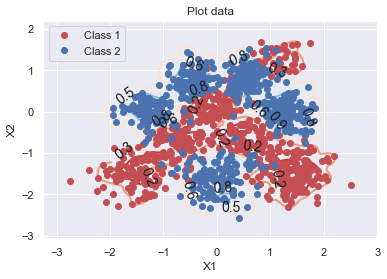
\includegraphics[width=0.3\paperwidth]{lap1}\hspace{1cm}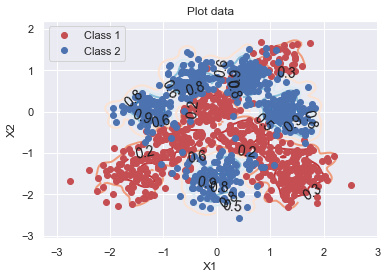
\includegraphics[width=0.3\paperwidth]{m1}
\par\end{centering}
\caption{Plots showing data and contour lines for the predictive distribution
generated by the Laplace approximation (left) and the MAP solution
(right).\label{fig:predictive_distributions} }
\end{figure}


\section{Exercise d)}

The final average training and test log-likelihoods are shown in Tables
\ref{tab:ll_MAP} and \ref{tab:ll_Laplace} . These results indicate that the models tend to overfit the data as explained in the previous section. Although, they would work well for data with low
variance, they will fail for highly varied data. Moreover, we can see that the Laplace log-likelihoods are smaller than the MAP solution, showing that although the model still overfits the data, it is less certain about its predictions than the MAP model.
\newline
The 2x2 confusion
matrices on the train and test set is shown in Tables \ref{tab:conf_MAP} and \ref{tab:conf_Laplace}.
By analising these tables, we conclude that, indeed, they are the same as predicted in Section \ref{a}. Both models compute their decision bounderies my minimizing the number of missclasifications.

\begin{table}[!h]
\centering{}%
\begin{minipage}[t]{0.5\textwidth}%
\begin{center}
\begin{tabular}{c|c}
\textbf{Avg. Train ll} & \textbf{Avg. Test ll}\tabularnewline
\hline 
-0.223 & -0.284\tabularnewline
\hline 
\end{tabular}\caption{Log-likelihoods for MAP solution.\label{tab:ll_MAP}}
\par\end{center}%
\end{minipage}%
\begin{minipage}[t]{0.5\textwidth}%
\begin{center}
\begin{tabular}{c|c}
\textbf{Avg. Train ll} & \textbf{Avg. Test ll}\tabularnewline
\hline 
-0.262 & -0.313\tabularnewline
\hline 
\end{tabular}\caption{Log-likelihoods for Laplace approximation.\label{tab:ll_Laplace}}
\par\end{center}%
\end{minipage}
\end{table}

\begin{table}[!h]
\centering{}%
\begin{minipage}[t]{0.5\textwidth}%
\begin{center}
\begin{tabular}{cc|c|c}
 & \multicolumn{1}{c}{} & \multicolumn{1}{c}{$\hat{y}$} & \tabularnewline
 &  & 0 & 1\tabularnewline
\cline{2-4} 
$y$ & 0 & 0.95 & 0.05\tabularnewline
\cline{2-4} 
 & 1 & 0.14 & 0.86\tabularnewline
\cline{2-4} 
\end{tabular} 
\par\end{center}
\caption{Conf. matrix for for MAP solution.\label{tab:conf_MAP}}
%
\end{minipage}%
\begin{minipage}[t]{0.5\textwidth}%
\begin{center}
\begin{tabular}{cc|c|c}
 & \multicolumn{1}{c}{} & \multicolumn{1}{c}{$\hat{y}$} & \tabularnewline
 &  & 0 & 1\tabularnewline
\cline{2-4} 
$y$ & 0 & 0.95 & 0.05\tabularnewline
\cline{2-4} 
 & 1 & 0.14 & 0.86\tabularnewline
\cline{2-4} 
\end{tabular} 
\par\end{center}
\caption{Conf. matrix for Laplace approximation.\label{tab:conf_Laplace}}
%
\end{minipage}
\end{table}


\section{Exercise e)}

In this exercise we aim to tune our parameters $ \sigma_0^2 $ and $ l $ by using a grid search. We construct a $ 10 \times 10 $ matrix representin all combination of $ \sigma_0^2 $ and $ l $. From coursework, we expect that the best value for $ l $ is in the interval of $ (0.1, 1) $ and we choose $ \sigma_0^2 $ in the interval of $ (0.1, 100) $. Moreover, we will choose logarithmically spaced values as we expect the model complexity to increase with the varience and therfore penalise our model evidence. The entries of the matrix will consist of the approximation of the model evidence and we will make use of a heat map to visualise our findings (See Figure \ref{fig:heat_map_plot}). The best model evidence corresponds to $ \sigma_0^2 = 1 $ and $ l = 0.6 $. It is worth noticing that the second best is very close and gives the values of $ \sigma_0^2 = 0.5 $ and $ l=0.5 $. The code used can be seen below.

\begin{verbatim}
l = np.geomspace(0.1, 1, num = 10)# XXX Width of the Gaussian basis funcction.
var = np.geomspace(0.1, 100, num = 10)

heat_map = np.ones((len(l), len(var)))

for m in range (len(l)):
    for n in range (len(var)):
        X_tilde_train = get_x_tilde(evaluate_basis_functions(l[m], X_train, X_train))
        	X_tilde_test = get_x_tilde(evaluate_basis_functions(l[m], X_test, X_train))

        wmap, fmap = train_wmap(var[n], X_tilde_train)
        S_0 = var[n] * np.identity(X_tilde_train.shape[ 1 ], dtype = float)
        Sn_inv = compute_hessian(X_tilde_train, wmap, var[n])

        heat_map[m][n] = log_model_evidence(fmap, Sn_inv, S_0)
        if(minim > heat_map[m][n]):
            minim = heat_map[m][n]
            m_prim = m
            n_prim = n

print("Optimized l, m: ({}, {})".format(l[m_prim], var(n_prim)))
ax = sns.heatmap(heat_map)
\end{verbatim}

Finally, from Figure \ref{fig:heat_map_plot} we can see how the model evidence is affected by our choice on the prior distibution. For very large variances the model complexity increases and penalises the model evidence.

\begin{figure}[!h]
\begin{centering}
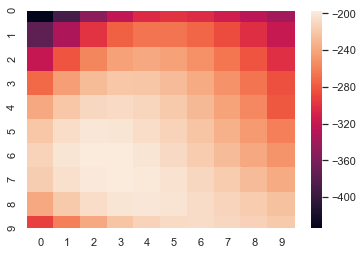
\includegraphics[width=0.3\paperwidth]{heatmap}
\par\end{centering}
\caption{Heat map plot of the the approximation of the model evidence obtained
in the grid search.\label{fig:heat_map_plot} }
\end{figure}

\newpage
\section{Exercise f)}

The training and test log-likelihoods per datapoint and confiusion matrix obtained for $ \sigma_0^2 = 1 $ and $ l = 0.6 $  can be seen in Tables \ref{tab:average_ll_after_tuning} and \ref{tab:confusion_after_tuning}. Figure \ref{fig:prediction_visualisation_after_tuning} displays the visualisation of the
contours of the resulting class predictive probabilities on top of the data after tuning the parameters. From these, we can clearly see the data separet by the expended bouderies. Moreover, the log-likelihoods show that this model fits and generalizes very well( the best we have seen so far including coursework). Furthermore, by looking at the confussion matrix we can see that this model predicts the data with higher accuracy than the previuos ones. 

\begin{figure}[!h]
\begin{centering}
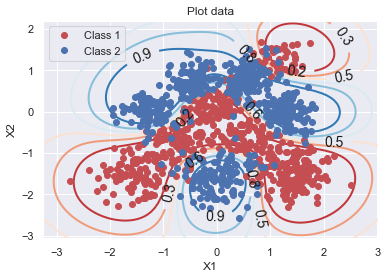
\includegraphics[width=0.3\paperwidth]{laplace2}
\par\end{centering}
\caption{Visualisation of the contours of the class predictive probabilities
for Laplace approximation after hyper-parameter tuning by maximising
the model evidence.\label{fig:prediction_visualisation_after_tuning} }
\end{figure}

\begin{table}[!h]
\centering{}%
\begin{minipage}[t]{0.4\columnwidth}%
\begin{center}
\vspace{-0.2cm}%
\begin{tabular}{c|c}
\textbf{Avg. Train ll} & \textbf{Avg. Test ll}\tabularnewline
\hline 
-0.198 & -0.176\tabularnewline
\hline 
\end{tabular} 
\par\end{center}
\caption{Average training and test log-likelihoods for Laplace approximation
after hyper-parameter tuning by maximising the model evidence.\label{tab:average_ll_after_tuning}}
%
\end{minipage}\hspace{2cm}%
\begin{minipage}[t]{0.4\columnwidth}%
\begin{center}
\begin{tabular}{cc|c|c}
 & \multicolumn{1}{c}{} & \multicolumn{1}{c}{$\hat{y}$} & \tabularnewline
 &  & 0 & 1\tabularnewline
\cline{2-4} 
$y$ & 0 & 0.96 & 0.04\tabularnewline
\cline{2-4} 
 & 1 & 0.09 & 0.91\tabularnewline
\cline{2-4} 
\end{tabular} 
\par\end{center}
\caption{Confusion matrix for Laplace approximation after hyper-parameter tuning
by maximising the model evidence.\label{tab:confusion_after_tuning}}
%
\end{minipage}
\end{table}


\section{Conclusions}
\begin{enumerate}
\item The Bayesian binary classifier performs better the simple RBF Logistic Classifier. Although, it requires more tuning on the choice of the prior and width. It can also computationally expansive as it requires the computation of determinants of high dimensional matrices. This can be improved by using optimized algorithms.
\item We do not need to know the normalization constant $ Z $ of the true distribution to apply the Laplace approximation.
\item For multimodal data we will need different Laplace approximations for each mode.
\item The Laplace approximation is that, since it is based on a Gaussian distribution, it is only directly applicable to real variables.
\item The Laplace approximationis based purely on the aspects of the true distribution at a specific value of the
variable, and so can fail to capture important global properties.
\end{enumerate}

\begin{thebibliography}
\bibitem{Patern recognition and machine learning}
Christopher M. Bishop
\textit{Patern recognition and machine learning} Spinger p.213-p.218
\end{thebibliography}

\end{document}
